\documentclass[10pt]{beamer}

\usepackage[utf8]{inputenc}
\usepackage{pgfpages}
\usepackage{dirtree}
\setbeamertemplate{note page}[plain]
\setbeameroption{show notes on second screen =left}
\AtEndNote{\vfill \begin{center} mm:hh \end{center}}
\newcommand{\notedir}[1] {
  \note{\dirtree{#1}}}
\def \ion {$^{\circ}$ }
\usepackage{tcolorbox}
\usepackage{tikz}
\usepackage{tikz-3dplot}
\usetikzlibrary{intersections,calc}
\usepackage{amsmath}
\usepackage{graphicx}
\usepackage{cases}

\def \heart {\textcolor{blue}{$\heartsuit$} }
\def \C {$\mathcal{C}$}


\tcbset{%
	basic/.style={colframe=black,
		      colback=white,
		      top= 0mm,
		      bottom = 2mm,
		      boxsep=0mm
		      }
}

    
\begin{document}  
    \beamertemplatenavigationsymbolsempty
    \setlength{\abovedisplayskip}{0pt}
    \setlength{\belowdisplayskip}{0pt}
    
    
    \frame{
	  
	  \frametitle{Q1 Juillet 2012.}
	  On considère un tétraèdre $ABCD$ et un plan parallèle à sa base $ABC$,
	  qui coupe les arêtes $[AD]$, $[BD]$ et $[CD]$ en des points notés respectivement $A'$ , $B'$ et $C'$.
	  Dans le triangle $ABC$, les milieux des côtés $[BC]$,
	  $[AC]$ et $[AB]$ sont respectivement notés $P$, $Q$ et $R$. \\
	  Démontrer que les droites $A'P$, $B'Q$ et $C'R$ sont concourantes.
	  \vfill
	  
	  \pause
	  % hypothèses et thèse
	  \begin{tcolorbox}[basic] 
	      \begin{columns}[t]
		 
		 \column{.5\textwidth}\centering
		      
		      \underline{Hypothèses} 
		      \begin{itemize}

		      \item $ABC\parallel A'B'C'$,
		      \item \begin{itemize}
		              \item[$\bullet$] $|AQ|=|QC|$,
		              \item[$\bullet$] $|AR|=|RB|$,
		              \item[$\bullet$] $|BP|=|PC|$.
		            \end{itemize}		            		              
		      \end{itemize}

		  
		  \column{.5\textwidth}\centering
		      
		      \underline{Thèse} \\		
		      \smallskip
		      $A'P,B'Q,C'R$ concourantes.
		
	      \end{columns}
	  \end{tcolorbox}
    \notedir{%
	.1 Énoncé.
	.2 Hypothèses (non visibles sur le dessin)..
	.2 Thèse : traduction mathématique..
	.2 Grand dessin.. 
	}
    }

    \frame{ 
	  % résolution ex1
	  \begin{columns}[t]
		\column{.5\textwidth}\centering 
		

			\underline{Dessin}\\
			
				  \begin{figure}[h]
				  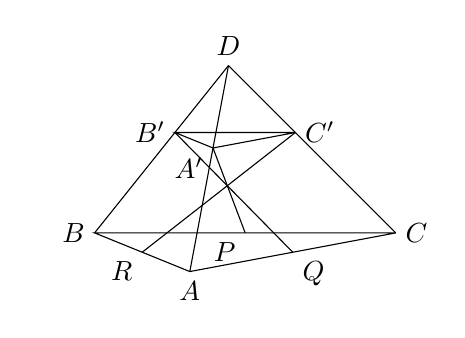
\begin{tikzpicture}[scale=0.85]				  
				  %\draw[help lines] (-3,-3,-3) grid (3,3,3);
				  %AXES
				  %\draw[->] (0,0,-3) -- (0,0,3) coordinate[label=below right:$z$]();
				  %\draw[->] (0,-3,0) -- (0,3,0) coordinate[label=above left:$y$]();
				  %\draw[->] (-3,0,0) -- (3,0,0) coordinate[label=above left:$x$]();
				  %TETRAEDRE et P,Q,R
				  \coordinate[label=below:$A$] (A) at (0,0,1.5);
				  \coordinate[label=left:$B$] (B) at (-2,0,0);
				  \coordinate[label=right:$C$] (C) at (2.5,0,0);
				  \coordinate[label=above:$D$] (D) at (0,2.5,0);
				\draw (A) -- (B) coordinate[pos=0.5,label=below left:$R$](R) -- (C) coordinate[pos=0.5,label=below left:$P$](P) -- (A) coordinate[pos=0.5,label=below right:$Q$](Q);
				  \draw[name path=AD] (A) -- (D);
				  \draw[name path=BD] (B) -- (D);
				  \draw[name path=CD] (C) -- (D);
				  %A',B',C'
				  \path[name path=x] (0,1.5,0) -- (3,1.5,0);
				  \path[name path=-x] (0,1.5,0) -- (-3,1.5,0);
				  \path[name path=z] (0,1.5,0) -- (0,1.5,3);
				  \path[name intersections={of=x and CD,by=C'}];
				  \coordinate[label=right:$C'$] () at (C');
				  \path[name intersections={of=-x and BD,by=B'}];
				  \coordinate[label=left:$B'$] () at (B');
				  \path[name intersections={of=z and AD,by=A'}];
				  \coordinate[label=below left:$A'$] () at (A');
				  %A'P,B'Q,C'R%
				  \draw (A') -- (P);
				  \draw (B') -- (Q);
				  \draw (C') -- (R);
				  
				  \draw (A') -- (B') -- (C') --cycle;
				  
				  \end{tikzpicture}
				  \end{figure}
			
				  \begin{tcolorbox}[basic] 
				      
				    \smallskip
				    \underline{Hypothèses} 
				    \begin{enumerate}

				    \item $ABC\parallel A'B'C'$,
				    \item \begin{itemize}
					      \item[$\bullet$] $|AQ|=|QC|$,
					      \item[$\bullet$] $|AR|=|RB|$,
					      \item[$\bullet$] $|BP|=|PC|$.
					  \end{itemize} 
				    \end{enumerate}
							      
				    \underline{Thèse} \\
				    \smallskip
				    $A'P,B'Q,C'R$ concourantes.
				    \end{tcolorbox}
		
		
		\column{.5\textwidth}\centering
		
		\underline{Résolution}\\ \flushleft
	
		\textit{Cas particulier (1): $ABC$ = $A'B'C'$} \\ \medskip		
		\heart Les médianes d'un triangle sont concourantes.
		\bigskip
		
		\textit{Cas particulier (2): $ABC$ contient $D$} \\ \medskip
		Les droites sont concourantes en D.
		\bigskip
		
		\textit{Cas général :} \\ \medskip
		
		\begin{enumerate}
		 \item $BC\parallel B'C'$,
		 \item $BC\parallel QR$ par Thalès.
		\end{enumerate}	\bigskip
		\centering $B'C'\parallel QR \rightarrow B'Q \nmid C'R$. \\ \medskip
		De la même façon : \\ \medskip $A'P\nmid C'R\text{ et }A'P\nmid B'Q$.
	   \end{columns}
       \notedir{%
	   .1 Prouver thèse.
	   .2 $A'P,B'Q,C'R$ concourantes.
	   .3 Cas particulier (1) $A'B'C'$ confondu avec $ABC$.
	   .3 Élément de théorie.
	   .4 Les médianes d'un $\Delta$ sont concourantes..
	   .3 Résolution..
	   .4 $A'P,B'Q,C'R$ médianes de $\Delta ABC$ $\rightarrow$ concourantes..
	   .3 Cas particulier (2) $A'B'C'$ contient $D$.
	   .4 $A'=B'=C'=D$ $\rightarrow A'P,B'Q,C'R$ concourantes..
	   .3 Cas général.
	   .4 Élément de théorie.
	   .5 3 droites non coplanaires sécantes 2 à 2 sont concourantes (à prouver car non vu)..
	   .4 Résolution.
	   .5 $BC$ parallèle à $B'C'$ car plans parallèles..
	   .5 $BC$ parallèle à $RC$ par Thalès dans $\Delta ABC$..
	   .5 $\rightarrow$ $B'C'$ parallèle à $RC$ par transitivité..
	   .6 $B',C',R,Q$ sont coplanaires..
	   .7 $B'Q$, $C'R$ sécantes car coplanaires et non $\parallel$..
	   .5 De la même façon, $A'P\nmid C'R$ et $A'P\nmid B'Q$..
	   .6 Les trois droites sont 2 à 2 sécantes..
	   }
       }
	  
       \frame{ 
       
	      \begin{columns}[t]
		\column{.5\textwidth}\centering 
		

			\underline{Dessin}\\
			
				  \begin{figure}[h]
				  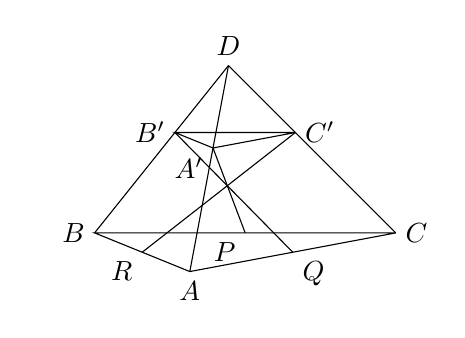
\begin{tikzpicture}[scale=0.85]				  
				  %\draw[help lines] (-3,-3,-3) grid (3,3,3);
				  %AXES
				  %\draw[->] (0,0,-3) -- (0,0,3) coordinate[label=below right:$z$]();
				  %\draw[->] (0,-3,0) -- (0,3,0) coordinate[label=above left:$y$]();
				  %\draw[->] (-3,0,0) -- (3,0,0) coordinate[label=above left:$x$]();
				  %TETRAEDRE et P,Q,R
				  \coordinate[label=below:$A$] (A) at (0,0,1.5);
				  \coordinate[label=left:$B$] (B) at (-2,0,0);
				  \coordinate[label=right:$C$] (C) at (2.5,0,0);
				  \coordinate[label=above:$D$] (D) at (0,2.5,0);
				\draw (A) -- (B) coordinate[pos=0.5,label=below left:$R$](R) -- (C) coordinate[pos=0.5,label=below left:$P$](P) -- (A) coordinate[pos=0.5,label=below right:$Q$](Q);
				  \draw[name path=AD] (A) -- (D);
				  \draw[name path=BD] (B) -- (D);
				  \draw[name path=CD] (C) -- (D);
				  %A',B',C'
				  \path[name path=x] (0,1.5,0) -- (3,1.5,0);
				  \path[name path=-x] (0,1.5,0) -- (-3,1.5,0);
				  \path[name path=z] (0,1.5,0) -- (0,1.5,3);
				  \path[name intersections={of=x and CD,by=C'}];
				  \coordinate[label=right:$C'$] () at (C');
				  \path[name intersections={of=-x and BD,by=B'}];
				  \coordinate[label=left:$B'$] () at (B');
				  \path[name intersections={of=z and AD,by=A'}];
				  \coordinate[label=below left:$A'$] () at (A');
				  %A'P,B'Q,C'R%
				  \draw (A') -- (P);
				  \draw (B') -- (Q);
				  \draw (C') -- (R);
				  
				  \draw (A') -- (B') -- (C') --cycle;
				  
				  \end{tikzpicture}
				  \end{figure}
			
				  \begin{tcolorbox}[basic] 
				      
				    \smallskip
				    \underline{Hypothèses} 
				    \begin{enumerate}

				    \item $ABC\parallel A'B'C'$,
				    \item \begin{itemize}
					      \item[$\bullet$] $|AQ|=|QC|$,
					      \item[$\bullet$] $|AR|=|RB|$,
					      \item[$\bullet$] $|BP|=|PC|$.
					  \end{itemize} 
				    \end{enumerate}
							      
				    \underline{Thèse} \\
				    \smallskip
				    $A'P,B'Q,C'R$ concourantes.
				    \end{tcolorbox}
		
		
		\column{.5\textwidth}\flushleft
		
		\bigskip 
		
		\begin{numcases}{}X= B'Q \cap C'R, \label{eq:1}\\
				  Y= A'P \cap C'R, \label{eq:2}\\
				  Z= A'P \cap B'Q. \label{eq:3} 
		\end{numcases} \medskip
		
		 
		\begin{align*}
		Y \in& C'R \subset B'C'R, \\
		Z \in& B'Q \subset B'C'R, \\
		\text{et }&  Y,Z \in A'P, \\[1em]				
			    Y =& Z  =A'P \cap B'C'R. \\[1.5em]		
			    Y =& A'P \cap C'R = A'P \cap B'Q, (\ref{eq:2}=\ref{eq:3}) \\
			      =& B'Q \cap C'R, \text{(transitivité)}\\
			      =& X.\\[0.5em]
			    X =& Y = Z. 	      
		\end{align*}
		\hfill $\qed$
	   \end{columns}
       
       \notedir{%
       .1 Prouver thèse.
       .2 Suite $A'P,B'Q,C'R$ concourantes.
       .3 Former un plan avec 2 droites, $C'R$ et $B'Q$.
       .4 L'intersect\ion de $A'P$ avec $C'R$ et celle avec $B'Q$\\ \hspace{5mm} appartiennent au plan et à $A'P$.
       .5 Ces deux intersect\ion sont confondues car point de \\ \hspace{5mm} percée de $A'P$ ds.~plan est unique..
       .6 Ce point de percée appartient à la fois à $A'P,B'Q,C'R \rightarrow$ droites concourantes.. 
       }
       }
  
\end{document}
